\subsubsection{モデルに基づく設計}

\term{モデルに基づく設計}{Model-Based Design, MBD} は、モデルを設計記録の中心に置く方法である。従来の文書中心の設計では、自然言語と非形式的な図を使うため、曖昧さや不完全さが残りやすい。また、必要な情報が複数文書に分散し、理解や分析が難しくなる。

モデルに基づく設計では、ツールが設計情報を整理し、表示し、分析できる。たとえば、モデルの一部をアニメーションやシミュレーションで確認したり、仮定を変えた場合の影響を調べたり、要求から設計、設計からテストへの追跡を支援したりできる。

\term{モデル駆動開発}{Model-Driven Development, MDD} は、モデルを開発プロセスの主要成果物として使い、コード生成や検証へつなげる考え方である。

\begin{figure}[htbp]
\centering
\IfFileExists{assets/generated_figures/ch03/fig-ch03-07.png}{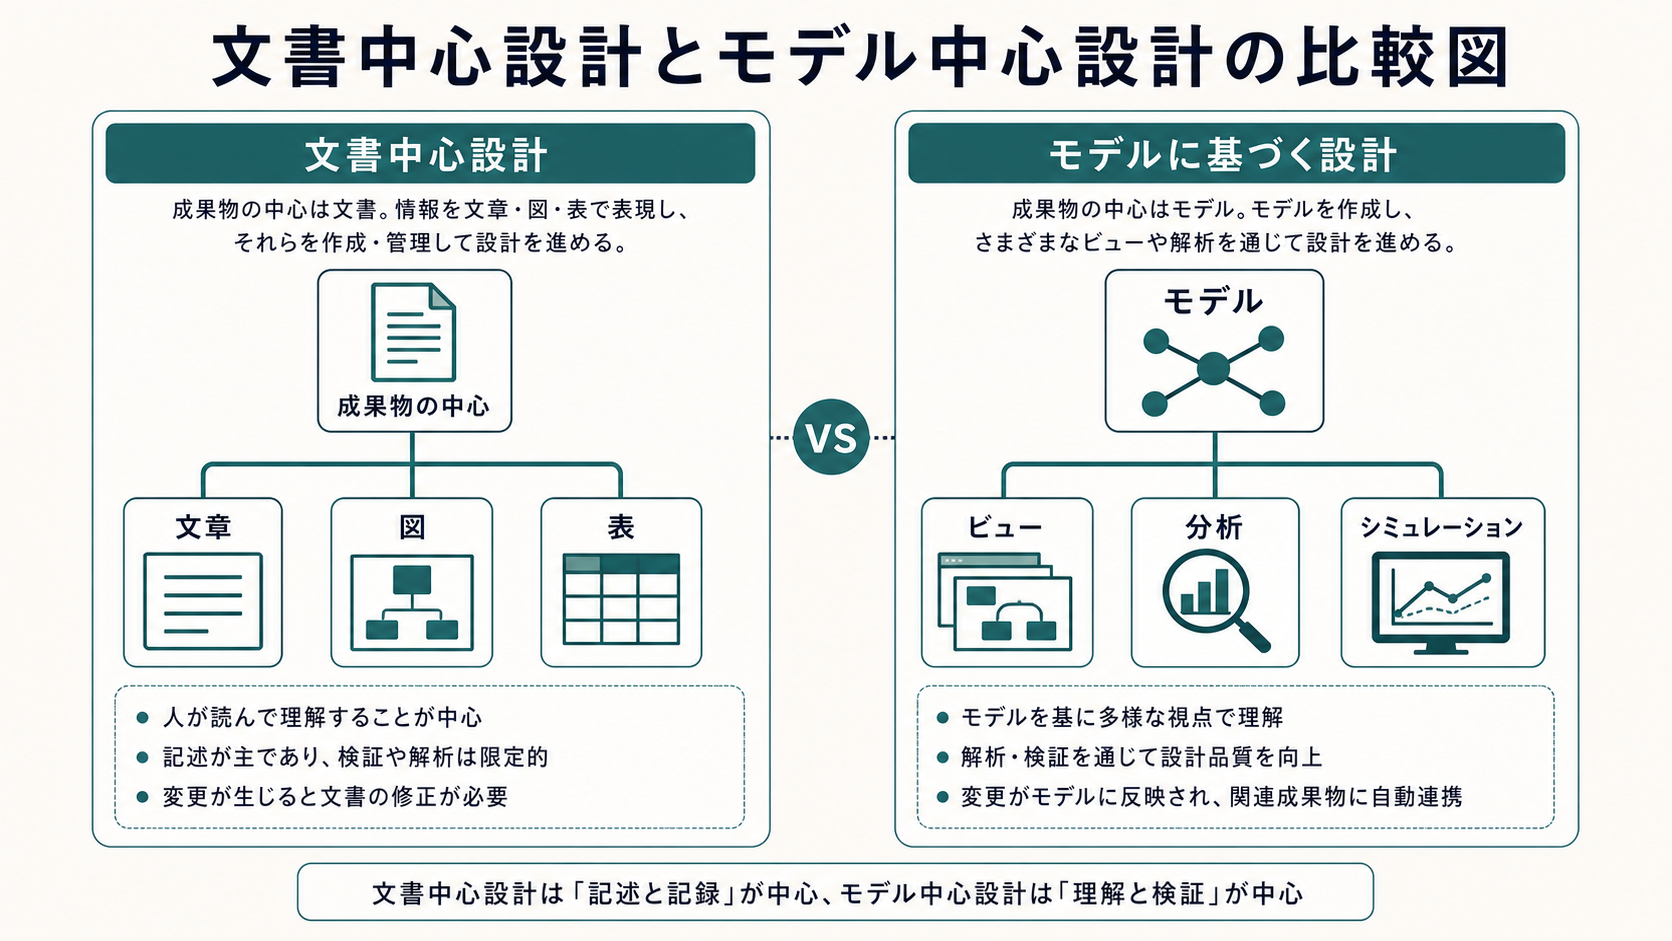
\includegraphics[width=0.96\linewidth]{assets/generated_figures/ch03/fig-ch03-07.png}}{\fbox{\parbox[c][48mm][c]{0.9\linewidth}{\centering 画像生成待ち\\文書中心設計とモデル中心設計の比較図}}}
\caption{文書中心設計とモデル中心設計の比較図}
\label{fig:ch03-07}
\end{figure}
